\chapter{Практичні результати}

У четвертому розділі представлено практичні результати
застосування алгоритму дифузії із сегментацією
та без із зазначенням вхідних даних.

\section{Результати експериментів}

Вихідні зображення для побудови карти глибин
за допомогою описаних алгоритмів були взяті з набору стереопар,
зроблених у Мідлберійському коледжі у 2001~\cite{middlebury:ds:2001},
2003~\cite{middlebury:ds:2003}
та 2006~\cite{middlebury:ds:2006:1}~\cite{middlebury:ds:2006:2} роках.
На рисунку \ref{fig:stereopair} наведені ліві та праві зображення зі стереопар,
для яких будувалися карти глибин у даному розділі дисертації,
а також істинні карти глибин.

\begin{figure}[h]
\centering
    \begin{subfigure}[t]{0.32\textwidth}
        \centering
        \includegraphics[width=\textwidth]{images/cloth_left}
    \end{subfigure}
    \hfill
    \begin{subfigure}[t]{0.32\textwidth}
        \centering
        \includegraphics[width=\textwidth]{images/pots_left}
    \end{subfigure}
    \hfill
    \begin{subfigure}[t]{0.32\textwidth}
        \centering
        \includegraphics[width=\textwidth]{images/poster_left}
    \end{subfigure}
    \vskip\baselineskip
    \begin{subfigure}[t]{0.32\textwidth}
        \centering
        \includegraphics[width=\textwidth]{images/cloth_right}
    \end{subfigure}
    \hfill
    \begin{subfigure}[t]{0.32\textwidth}
        \centering
        \includegraphics[width=\textwidth]{images/pots_right}
    \end{subfigure}
    \hfill
    \begin{subfigure}[t]{0.32\textwidth}
        \centering
        \includegraphics[width=\textwidth]{images/poster_right}
    \end{subfigure}
    \vskip\baselineskip
    \begin{subfigure}[t]{0.32\textwidth}
        \centering
        \includegraphics[width=\textwidth]{images/cloth_ground_truth}
        \caption{Тканина (Cloth1), $400 \times 355$ пікселів}
    \end{subfigure}
    \hfill
    \begin{subfigure}[t]{0.32\textwidth}
        \centering
        \includegraphics[width=\textwidth]{images/pots_ground_truth}
        \caption{Квіткові горщики (Flowerpots), $400 \times 338$ пікселів}
    \end{subfigure}
    \hfill
    \begin{subfigure}[t]{0.32\textwidth}
        \centering
        \includegraphics[width=\textwidth]{images/poster_ground_truth}
        \caption{Плакат (Poster), $400 \times 352$ пікселів}
    \end{subfigure}
    \caption{Зображення стереопар,
             для яких будувалися карти глибин у цьому розділі.
             Перший рядок містить ліві зображення, другий~---~праві,
             третій~---~істинні карти глибин}
    \label{fig:stereopair}
\end{figure}

На рисунку \ref{fig:result:pixel} зображені карти глибин,
отримані за допомогою алгоритму дифузії,
де кожній долі графу відповідає один піксель,
як описано в другому розділі дисертації.
Для кожного зображення вказано кількість ітерацій, зроблених алгоритмом дифузії,
час виконання всіх ітерацій, а також кількість міток $\left| D \right|$ в об'єктах графу.

\begin{figure}[h]
\centering
    \begin{subfigure}[t]{0.32\textwidth}
        \centering
        \includegraphics[width=\textwidth]{images/cloth_pixel_based_stereo}
        \caption{$2'400$ ітерацій, $5$ годин $40$ хвилин, $\left| D \right| = 40$}
        \label{fig:cloth:pixel}
    \end{subfigure}
    \hfill
    \begin{subfigure}[t]{0.32\textwidth}
        \centering
        \includegraphics[width=\textwidth]{images/pots_pixel_based_stereo}
        \caption{$2'800$ ітерацій, $1$ година $20$ хвилин, $\left| D \right| = 16$}
        \label{fig:flowerpots:pixel}
    \end{subfigure}
    \hfill
    \begin{subfigure}[t]{0.32\textwidth}
        \centering
        \includegraphics[width=\textwidth]{images/poster_pixel_based_stereo}
        \caption{$1'600$ ітерацій, $46$ хвилин, $\left| D \right| = 16$}
        \label{fig:poster:pixel}
    \end{subfigure}
    \caption{Карти глибин, отримані алгоритмом дифузії без сегментації зображення}
    \label{fig:result:pixel}
\end{figure}

На рисунку \ref{fig:result:superpixel} зображені карти глибин,
отримані за допомогою алгоритму дифузії з використанням сегментації зображення,
що описана в попередньому розділі дисертації,
з розміром комірок $5$ на $5$ пікселів.
Для кожного зображення вказано кількість ітерацій, зроблених алгоритмом дифузії,
час виконання всіх ітерацій, а також кількість міток $\left| D \right|$ в об'єктах графу.
Отримані досить гладкі карти глибин,
однак видніються неточності на краях об'єктів.

\begin{figure}[h]
\centering
    \begin{subfigure}[t]{0.32\textwidth}
        \centering
        \includegraphics[width=\textwidth]{images/cloth_superpixel_based_stereo}
        \caption{$100$ ітерацій, $19$ хвилин, $\left| D \right| = 40$}
        \label{fig:cloth:superpixel}
    \end{subfigure}
    \hfill
    \begin{subfigure}[t]{0.32\textwidth}
        \centering
        \includegraphics[width=\textwidth]{images/pots_superpixel_based_stereo}
        \caption{$450$ ітерацій, $15$ хвилин, $\; \left| D \right| = 16$}
        \label{fig:flowerpots:superpixel}
    \end{subfigure}
    \hfill
    \begin{subfigure}[t]{0.32\textwidth}
        \centering
        \includegraphics[width=\textwidth]{images/poster_superpixel_based_stereo}
        \caption{$400$ ітерацій, $14$ хвилин, $\; \left| D \right| = 16$}
        \label{fig:poster:superpixel}
    \end{subfigure}
    \caption{Карти глибин, отримані алгоритмом дифузії після сегментації зображення}
    \label{fig:result:superpixel}
\end{figure}

Алгоритм був реалізований на мові програмування Rust.
В ході роботи був використаний комп'ютер з процесором
Intel(R) Core(TM) i5-7400 і оперативно запам'ятовуючим пристроєм DDR4 2133MHz.

Для порівняння на рисунку \ref{fig:result:dynamic}
наведені карти глибин,
отримані з тими самими штрафними функціями
та значеннями параметрів за допомогою динамічного програмування,
де для кожного рядка зображення карта глибин шукається незалежно.
На отриманих картах глибин чітко видно горизонтальні лінії,
які є результатом того, що всі рядки зображення обробляються незалежно.
Даний метод описано в першому розділі дисертації.

\begin{figure}[h]
\centering
    \begin{subfigure}[t]{0.32\textwidth}
        \centering
        \includegraphics[width=\textwidth]{images/cloth_dynamic_result}
    \end{subfigure}
    \hfill
    \begin{subfigure}[t]{0.32\textwidth}
        \centering
        \includegraphics[width=\textwidth]{images/pots_dynamic_result}
    \end{subfigure}
    \hfill
    \begin{subfigure}[t]{0.32\textwidth}
        \centering
        \includegraphics[width=\textwidth]{images/poster_dynamic_result}
    \end{subfigure}
    \caption{Карти глибин, отримані за допомогою динамічного програмування}
    \label{fig:result:dynamic}
\end{figure}

\section{Залежність від розміру комірок}

Як показано в попередньому розділі дисертації у формулі
\eqref{eq:diffusion:superpixel:complexity},
зі збільшенням розміру комірок, на які розбивається зображення,
зменшується складність виконання ітерацій алгоритму дифузії.
На рисунку \ref{fig:superpixel:cloth:cell:size}
показані карти глибин для однієї й тієї ж стереопари,
отримані алгоритмом дифузії з використанням суперпікселів,
але при розділенні зображення на комірки різного розміру.
З рисунку видно, що при збільшенні розміру комірок зменшується час,
необхідний на розв'язання задачі оптимізації алгоритмом дифузії,
однак водночас побудована карта глибин стає менш гладкою,
додаються артефакти на краях об'єктів.
Вони можуть бути незначними для гладких зображень, як тканина,
але для зображень, які містять дрібніші об'єкти,
погіршення можуть бути суттєвими.
Прикладом може слугувати рисунок \ref{fig:superpixel:tsukuba:cell:size},
на якому видно, що камера змінює свою форму,
а на границях лампи з'являється все більше артефактів при збільшенні розміру комірок.

\begin{figure}[h]
\centering
    \begin{subfigure}[t]{0.32\textwidth}
        \centering
        \includegraphics[width=\textwidth]{images/cloth_superpixel_2}
        \caption{Розмір комірки $2\times 2$ пікселі,
                 $400$ ітерацій,
                 $3$ години $20$ хвилин}
    \end{subfigure}
    \hfill
    \begin{subfigure}[t]{0.32\textwidth}
        \centering
        \includegraphics[width=\textwidth]{images/cloth_superpixel_based_stereo}
        \caption{Розмір комірки $5 \times 5$ пікселів,
                 $100$ ітерацій,
                 $19$ хвилин}
    \end{subfigure}
    \hfill
    \begin{subfigure}[t]{0.32\textwidth}
        \centering
        \includegraphics[width=\textwidth]{images/cloth_superpixel_8}
        \caption{Розмір комірки $8\times 8$ пікселів,
                 $5$ ітерацій,
                 $45$ секунд}
    \end{subfigure}
    \caption{Залежність якості карти глибин від розмірів комірок.
             Для всіх випадків $\left| D \right| = 40$, $\alpha = 1.4$}
    \label{fig:superpixel:cloth:cell:size}
\end{figure}

\begin{figure}[h]
\centering
    \begin{subfigure}[t]{0.4\textwidth}
        \centering
        \includegraphics[width=\textwidth]{images/tsukuba_left}
        \caption{Ліве зображення}
    \end{subfigure}
    \begin{subfigure}[t]{0.4\textwidth}
        \centering
        \includegraphics[width=\textwidth]{images/tsukuba_ground_truth}
        \caption{Істинна карта глибин}
    \end{subfigure}
    \vskip\baselineskip
    \begin{subfigure}[t]{0.32\textwidth}
        \centering
        \includegraphics[width=\textwidth]{images/tsukuba_superpixel_5}
        \caption{Розмір комірки $5\times 5$ пікселів,
                 $310$ ітерацій,
                 $8$ хвилин}
    \end{subfigure}
    \hfill
    \begin{subfigure}[t]{0.32\textwidth}
        \centering
        \includegraphics[width=\textwidth]{images/tsukuba_superpixel_8}
        \caption{Розмір комірки $8 \times 8$ пікселів,
                 $200$ ітерацій,
                 $4$ хвилини}
    \end{subfigure}
    \hfill
    \begin{subfigure}[t]{0.32\textwidth}
        \centering
        \includegraphics[width=\textwidth]{images/tsukuba_superpixel_12}
        \caption{Розмір комірки $12\times 12$ пікселів,
                 $100$ ітерацій,
                 $2$ хвилини}
    \end{subfigure}
    \caption{Залежність якості карти глибин від розмірів комірок.
             Для всіх випадків $\left| D \right| = 15$, $\alpha = 10$.
             Розмір зображення $384$ на $288$ пікселів}
    \label{fig:superpixel:tsukuba:cell:size}
\end{figure}

\section{Штрафні функції}

У якості штрафної функції для вершин $f$
в даній роботі використовувався модуль різниці
інтенсивностей відповідних пікселів на двох зображеннях
\begin{equation*}
    f_{\left(x, y \right)} \left( d \right) =
    \left| L \left(x, y \right) - R \left(x - d, y \right) \right|,
\end{equation*}
де $\left(x, y \right) \in T$, $d \in D$,
а в якості штрафної функції для дужок $g$~---~модуль різниці обраних зсувів
$d \in D$ та $d' \in D$ в сусідніх об'єктах графу
\begin{equation*}
    g_{\left(x, y \right), \left(x', y' \right)} \left(d, d' \right) =
    \alpha \cdot \left| d - d' \right|,
\end{equation*}
де $\left(\left(x, y \right), \left(x', y' \right) \right) \in \mathcal{N}$,
а $\alpha = 1.4$~---~коефіцієнт згладжування,
підібраний експериментальним шляхом.
У попередньому розділі вказано, що
$\left| d - d' \right|$~---~субмодулярна функція від величин
$d, d' \in D$.
Після домноження на константу $\alpha \in \mathbb{R}$
функція залишається субмодулярною,
що гарантує існування розмітки після розв'язання оптимізаційної задачі
алгоритмом дифузії.

\section{Додаткові обмеження}

Додатково були введені обмеження на можливі мітки в кожному об'єкті:
для об'єкта $\left( x, y \right) \in T$ з горизонтальною координатою $x$
не може бути обраний зсув $d \in D$ такий, що $d > x$,
який би перевів горизонтальну координату пікселя у від'ємне число
$x - d < 0$ (рис.~\ref{fig:disparity:restriction:vertex}).
Дані обмеження були введені за допомогою штрафної функції $f$
\begin{equation*}
    f_{\left(x, y \right)} \left( d \right) =
    \begin{cases}
        \left| L \left(x, y \right) - R \left(x - d, y \right) \right|,
            & x \ge d, \\
        + \infty, & x < d.
    \end{cases}
\end{equation*}

\begin{figure}[h]
  \centering
  \includegraphics[width=0.9\textwidth]{images/disparity_restriction_vertex}
  \caption{Обмеження на вибір мітки в об'єкті.
           $L_j$ та $R_j$~---~рядок під номером $j$
           лівого та правого зображення відповідно.
           Допустимі зсуви $d \in \left\{0, 1, 2, 3 \right\}$
           для даного об'єкта $\left(i, j \right)$
           з горизонтальною координатою $i = 3$
           зображено чорними стрілками,
           недопустимі зсуви $d > 3$~---~червоною стрілкою}
  \label{fig:disparity:restriction:vertex}
\end{figure}

Також були накладені обмеження на зсуви в сусідніх об'єктах по горизонталі:
$d' \le d + 1$ (рис.~\ref{fig:disparity:restriction:edge}),
де $d \in D$~---~мітка в об'єкті $\left(x, y \right) \in T$,
$d'$~---~мітка в об'єкті
$\left(x', y' \right) \in \mathcal{N} \left(x, y \right)$
такому, що $x' = x + 1$.

\begin{figure}[h]
  \centering
  \includegraphics[width=0.9\textwidth]{images/disparity_restriction_edges}
  \caption{Обмеження на вибір міток у сусідніх об'єктах по горизонталі.
           $L_j$ та $R_j$~---~рядок під номером $j$
           лівого та правого зображення відповідно.
           Чорною стрілкою позначено обраний зсув $d \in D$ для об'єкту
           $\left(i, j \right)$.
           Синіми стрілками позначені допустимі зсуви $d'$
           для об'єкта $\left(i + 1, j \right)$ такі, що $d' \le d + 1$,
           недопустимі зсуви $d' > d + 1$ позначено червоними стрілками}
  \label{fig:disparity:restriction:edge}
\end{figure}

\section*{Висновки до розділу 4}
\addcontentsline{toc}{section}{Висновки до розділу 4}

У даному розділі наведено приклади роботи алгоритму
з використанням запропонованого методу прискорення алгоритмів стереобачення,
що використовує сегментацію зображення.
Наведено штрафні функції та інші параметри алгоритму, які буди використані.
З експериментів видно, що запропонований метод дійсно прискорює роботу алгоритму дифузії,
зменшуючи необхідну кількість ітерацій та їх складність,
водночас знижуючи якість побудованої карти глибин у деяких випадках.
